\section{INTRODUCTION}
This document presents the document of the final project developed for the "Embedded platforms and communications for \acrfullr{iot}".

The final project consist on the design, integration, implementation and validation of a IoT system to control biological data and other parameters like the GPS location of plants that have unique characteristics such as bonsais. This will allow farmers and 
producers to detect early problems in crops, problems in the soil or in the transportation of the plants. 

This system is centered around a embedded solution based on \texttt{ARM Cortex M0+}, with low power consumption and all the capabilities needed to cover the requirements. Also, several sensors are used and integrated in the design to obtain all the previous parameters mentioned. Different connections 
such as \texttt{\acrfullr{i2c}} and \texttt{\acrfullr{uart}} are used to communicate these elements with the \texttt{CPU}. With the usage of \texttt{Mbed-OS}, a thread-based software 
solution is used to achieve all the functionalities.

Finally, the complete solution is presented in \autoref{fig:solutionIntro}. In the center, the microcontroller connects to two protoboards:
\begin{itemize}
    \item The left one includes a moisture sensor, a phototransistor and a RGB Led, powered by 3.3V.
    \item The Right one includes the accelerometer, the color sensor, the temperature and humidity sensor and the GPS, powered by 5V.
\end{itemize}

\begin{figure}[H]
    \centering
    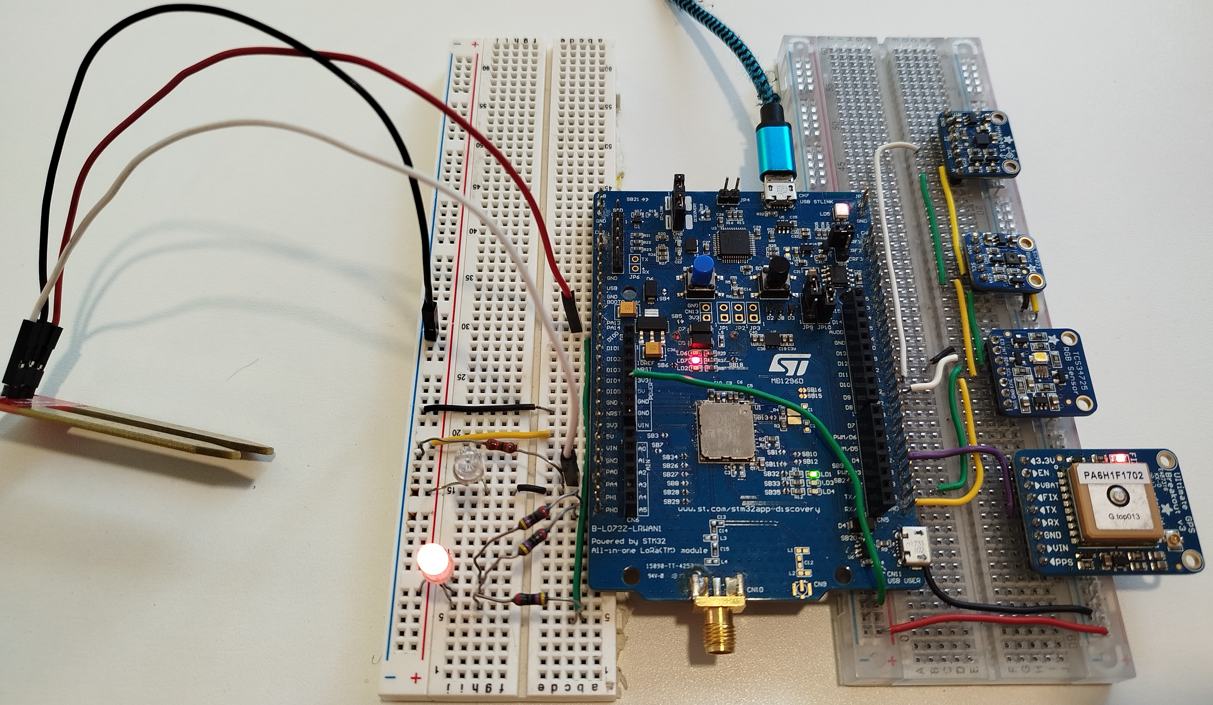
\includegraphics[width=1\textwidth]{images/1/sistema.png}
    \caption{Final solution developed}
    \label{fig:solutionIntro}
\end{figure}